\subsection{Mean Squared Error Loss (MSE)}\label{subsec:mse}

La \textbf{Mean Squared Error Loss (MSE)} è una funzione di perdita ampiamente utilizzata per i modelli di regressione, particolarmente quando i dati sono distribuiti secondo una \textbf{distribuzione gaussiana}. Essa misura la media dei quadrati delle differenze tra i valori osservati e quelli predetti dal modello.

\begin{definizione}{MSE}{mse}
La \textbf{MSE} per \( n \) osservazioni è definita come:
\[
\mathrm{MSE} = \frac{1}{n} \sum_{i=1}^n \left( y_i - \hat{y}_i \right)^2
\]
dove \( y_i \) è il valore osservato e \( \hat{y}_i \) è il valore predetto dal modello.
\end{definizione}

\subsubsection*{Distribuzione dei dati}

Nel contesto dei dati Gaussiani, supponiamo che \( Y(i) \) sia distribuito come \( Y(i) \sim \mathcal{N}(\mu(i), \sigma^2(i)) \), con \( \mu(i) \) e \( \sigma(i) \) dipendenti dal parametro \( x(i) \).

La funzione di verosimiglianza per \( n \) osservazioni è quindi:

\[
\ell(\mu(i), \sigma(i)) = \sum_{i=1}^n \left[-\log(\sqrt{2\pi}) -\log(\sigma(i)) - \frac{(y(i) - \mu(i))^2}{2\sigma(i)^2} \right]
\]
Dove:
\begin{itemize}
    \item \( \mu(i) \) è la media prevista,
    \item \( \sigma(i) \) è la deviazione standard prevista per il dato \( i \).
\end{itemize}

\subsubsection{I casi}

\begin{itemize}
    \item \textbf{Caso 1: Nessuna dipendenza dall'input (\Cref{ex:mle-norm})}: Se non c'è dipendenza da \( x(i) \), la funzione di log-verosimiglianza diventa:
        \[
            \ell(\mu, \sigma) = C - n \log \sigma - \frac{1}{2\sigma^2} \sum_{i=1}^n (y(i) - \mu)^2
        \]
        Risolvendo, otteniamo lo stimatore per la media e la deviazione standard:
        \[
            \hat{\mu} = \frac{1}{n} \sum_{i=1}^n y(i), \quad \hat{\sigma}^2 = \frac{1}{n} \sum_{i=1}^n (y(i) - \hat{\mu})^2
        \]

    \item \textbf{Caso 2: Modello regressivo con varianza costante (\textit{omoschedastico})}: Se la deviazione standard \( \sigma(i) \) è costante, e i parametri \( \mu(i) \) dipendono da \( x(i) \), possiamo assumere una relazione parametrica. Ad esempio, un modello lineare potrebbe essere usato per descrivere:
        \[
            \sigma(i) = \sigma, \quad \mu(i) = \nu(x(i); \vec{\alpha})
        \]
        La funzione di log-verosimiglianza diventa:
        \[
            \ell(\sigma, \vec{\alpha}) = C - n \log \sigma - \frac{1}{2\sigma^2} \sum_{i=1}^n (y(i) - \nu(x(i); \vec{\alpha}))^2
        \]
        Introduciamo la funzione \textbf{SE} (\textit{Squared Error}) che calcola la differenza al quadrato degli argomenti:
        \[
            \mathrm{SE}(y, z) = (y - z)^2
        \]
        Questo permette di riscrivere la log-verosimiglianza in funzione della
        MSE (\Cref{def:mse}):
        \[
            \mathrm{loss}_{\text{MSE}}(\vec{\alpha}) = \frac{1}{n} \sum_{i=1}^n \mathrm{SE}(y(i), \nu(x(i); \vec{\alpha})) = \frac{1}{n} \sum_{i=1}^n (y(i) - \nu(x(i); \vec{\alpha}))^2
        \]
        \[
            \Rightarrow \ell(\sigma, \vec{\alpha}) = C - n \log \sigma - \frac{1}{2\sigma^2}
            n\,\mathrm{loss}_{\text{MSE}}(\vec{\alpha})
            = C - n (\log \sigma + \frac{1}{2\sigma^2}
            \mathrm{loss}_{\text{MSE}}(\vec{\alpha}))
        \]
        Da qui si ottiene lo stimatore \( \hat{\sigma} \):
        \[
            \hat{\sigma} = \sqrt{\mathrm{loss}_{\text{MSE}}(\vec{\alpha})}
        \]
        L'ottimizzazione degli altri parametri segue dalla minimizzazione della
        \( \mathrm{loss}_{\text{MSE}} \).

        \begin{nota}{$\mathrm{loss_{MSE}}$}{}
            La funzione $\mathrm{loss_{MSE}}$ è semplicemente definita come lo
            \textbf{scarto quadratico medio} tra i valori osservati e quelli
            predetti dal modello.
        \end{nota}

    \item \textbf{Caso 3: Dipendenza da \( x \)}: Se i parametri \( \mu(i) \) e \( \sigma(i) \) dipendono da \( x(i) \), possiamo definire la funzione di regressione come segue:
        \[
            \mu(i) = \nu(x(i); \vec{\alpha}), \quad \sigma(i) = \tau(x(i); \vec{\alpha})
        \]
        Dove \( \nu(x(i); \vec{\alpha}) \) è il modello di regressione e \( \tau(x(i); \vec{\alpha}) \) è la variabilità associata.

        \begin{nota}{Stima di $\vec{\alpha}$}{}
            Questa funzione viene ottimizzata usando metodi iterativi, come la discesa
            del gradiente, per trovare i migliori parametri.
        \end{nota}
\end{itemize}

\section{Regressione Lineare Semplice}\label{sec:regressione}

La \textbf{regressione lineare semplice} è uno dei modelli più basilari in statistica e machine learning. In questo caso, si cerca di modellare la relazione tra una variabile dipendente \( Y \) e una variabile indipendente \( X \).

\subsection{Modello e parametri}

Il modello della regressione lineare semplice assume che la variabile dipendente \( Y \) sia una combinazione lineare della variabile indipendente \( X \), più un errore \( \epsilon \). In altre parole:
\[
Y_i = \beta_0 + \beta_1 X_i + \epsilon_i
\]
dove:
\begin{itemize}
\item \( Y_i \) è la variabile dipendente (osservazione), che si assume essere normalmente distribuita: 
    \[ Y_i \sim \mathcal{N}(\beta_0 + \beta_1 X_i, \sigma^2), \]
\item \( X_i \) è la variabile indipendente, che viene trattata come una variabile deterministica (osservata),
\item \( \beta_0 \) è l'intercetta del modello,
\item \( \beta_1 \) è la pendenza della retta di regressione,
\item \( \epsilon_i \) è l'errore, che si assume essere normalmente distribuito con media zero e varianza costante \( \sigma^2 \):
        \[ \epsilon_i \sim \mathcal{N}(0, \sigma^2). \]
\end{itemize}

\begin{figure}[H]
    \centering
    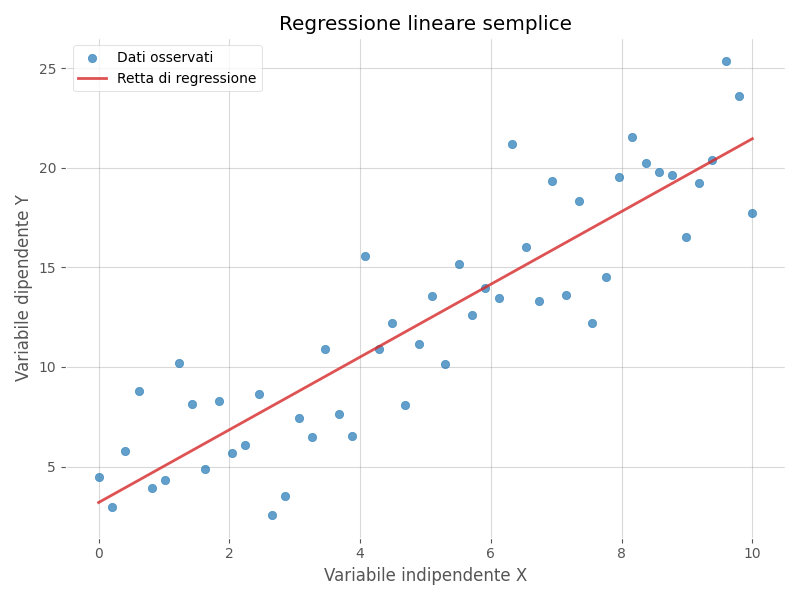
\includegraphics[width=0.6\textwidth]{images/th_16_18/regressione_lineare_semplice.png}
    \caption{Esempio di regressione lineare semplice. La retta di regressione approssima la relazione tra la variabile indipendente \( X \) e la variabile dipendente \( Y \).}
    \label{fig:regressione_lineare_semplice}
\end{figure}

Il modello descrive una \textbf{retta di regressione} che approssima la relazione tra \( X \) e \( Y \).

\begin{definizione}{Parametri del modello}{regressione-lineare-parametri}
I parametri del modello di regressione lineare sono \( \beta_0 \) (intercetta), \( \beta_1 \) (pendenza), e \( \sigma^2 \) (varianza dell'errore).
\end{definizione}

\begin{nota}{Assunzioni del modello}{reg-lin-assunzioni}
Il modello di regressione lineare semplice assume che:
\begin{itemize}
    \item La relazione tra \( X \) e \( Y \) sia lineare.
    \item Gli errori \( \epsilon_i \) siano indipendenti e normalmente distribuiti con media zero e varianza costante (\( \sigma^2 \)).
    \item La variabile dipendente \( Y \) segue una distribuzione normale con media \( \mu = \beta_0 + \beta_1 X_i \) e varianza costante \( \sigma^2 \): \( Y_i \sim \mathcal{N}(\beta_0 + \beta_1 X_i, \sigma^2) \).
    \item La variabile indipendente \( X \) è deterministica, mentre la variabile dipendente \( Y \) è casuale.
\end{itemize}
\end{nota}

\begin{nota}{Baricentro della regressione}{regressione-baricentro}
Il \textbf{baricentro} della regressione è il punto medio dei dati osservati, dato dalla media di \( X \) e \( Y \). In termini matematici, il baricentro \( (\overline{x}, \overline{y}) \) è dato da:
\[
\overline{x} = \frac{1}{n} \sum_{i=1}^n x_i, \quad \overline{y} = \frac{1}{n} \sum_{i=1}^n y_i
\]
\end{nota}

\begin{figure}[H]
    \centering
    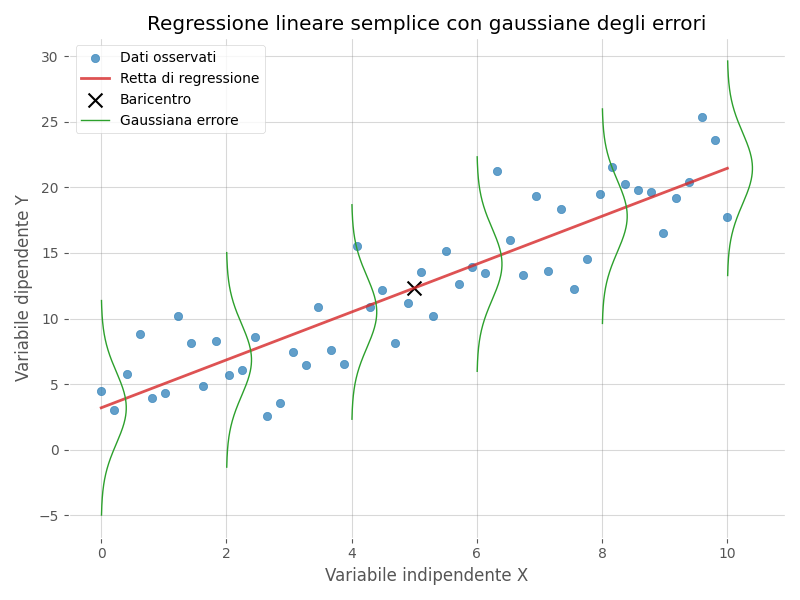
\includegraphics[width=0.6\textwidth]{images/th_16_18/regressione_lineare_semplice2.png}
    \caption{Esempio di regressione lineare semplice con retta passante per il baricentro dei dati e curve di distribuzione gaussiana degli errori attorno alla retta.}
    \label{fig:regressione_lineare_semplice_gaussianine_e_baricentro}
\end{figure}

\subsection{Stima dei parametri tramite Maximum Likelihood (MLE)}

I parametri \( \beta_0 \), \( \beta_1 \), e \( \sigma^2 \) possono essere stimati utilizzando il metodo della massima verosimiglianza (MLE). La funzione di log-verosimiglianza è:

\[
\ell(\beta_0, \beta_1, \sigma) = C - n \log \sigma - \frac{1}{2\sigma^2} \sum_{i=1}^n (y_i - \beta_0 - \beta_1 x_i)^2
\]

Per trovare i parametri che massimizzano la log-verosimiglianza, possiamo derivare rispetto ai parametri e risolvere il sistema di equazioni. I parametri stimati risultano:

\begin{definizione}[
    enhanced,
    overlay last={
        \node[anchor=south east, font=\large, text=cs@definition] at (frame.south east) {$\bigstar$};
    }
]{Stima della pendenza}{regressione-lineare-pendenza}
    Lo stimatore per la pendenza \( \hat{\beta}_1 \) nel modello di regressione lineare è dato dalla seguente espressione:
    \[
        \hat{\beta}_1 = \frac{\overline{xy} - \overline{x}\, \overline{y}}{\overline{x^2} - \overline{x}^2}
    \]
    dove:
    \begin{itemize}
        \item \( \overline{x} = \frac{1}{n} \sum_{i=1}^n x_i \) è la media dei valori di \( x \),
        \item \( \overline{y} = \frac{1}{n} \sum_{i=1}^n y_i \) è la media dei valori di \( y \),
        \item \( \overline{xy} = \frac{1}{n} \sum_{i=1}^n x_i y_i \) è la media dei prodotti \( x_i y_i \),
        \item \( \overline{x^{2}} = \frac{1}{n} \sum_{i=1}^n x_i^2 \) è la media dei quadrati dei valori di \( x \).
    \end{itemize}
\end{definizione}
Questa formula fornisce la stima ottimale della pendenza \( \hat{\beta}_1 \) nel
caso di regressione lineare semplice.

\begin{definizione}[
    enhanced,
    overlay last={
        \node[anchor=south east, font=\large, text=cs@definition] at (frame.south east) {$\bigstar$};
    }
]{Stima dell'intercetta}{regressione-lineare-intercetta}
    La stima per l'intercetta \( \hat{\beta}_0 \) è data dalla formula:
    \[
        \hat{\beta}_0 = \overline{y} - \hat{\beta}_1 \overline{x}
    \]
    Dove:
    \begin{itemize}
        \item \( \overline{x} \) è la media dei valori di \( X \),
        \item \( \overline{y} \) è la media dei valori di \( Y \),
        \item \( \hat{\beta}_1 \) è la pendenza della retta di regressione.
    \end{itemize}
\end{definizione}

La retta di regressione \( \hat{y} = \hat{\beta}_0 + \hat{\beta}_1 x \) è costruita in modo che minimizzi la somma dei quadrati degli errori tra i valori osservati e quelli predetti. Un risultato interessante della regressione lineare è che questa retta passa sempre per il \textbf{baricentro} il  dei dati, dato dalle medie \( \overline{x} \) e \( \overline{y} \).

\begin{dimostrazione}{Baricentro appartiene alla regressione lineare}{}
Per \( x = \overline{x} \), la retta di regressione assume il valore:
\[
\hat{y}(\overline{x}) = \hat{\beta}_0 + \hat{\beta}_1 \overline{x}
\]
Sostituendo \( \hat{\beta}_0 = \overline{y} - \hat{\beta}_1 \overline{x} \) nella formula della retta otteniamo:
\[
\hat{y}(\overline{x}) = \left( \overline{y} - \hat{\beta}_1 \overline{x} \right) + \hat{\beta}_1 \overline{x} = \overline{y}
\]
\end{dimostrazione}

\begin{dimostrazione}{Calcolo degli stimatori \( \beta_0 \) e \( \beta_1 \)}{calcolo-b1-b0}

Partiamo dalla funzione di perdita MSE, che nel caso della regressione lineare è definita come:
\[
\text{loss}_{\text{MSE}} (\hat{\beta_0}, \hat{\beta_1}) = \frac{1}{n} \sum_{i=1}^n \left( y_i - \hat{y}_i \right)^2
\]
dove \( \hat{y}_i = \hat{\beta_0} + \hat{\beta_1} x_i \) sono i valori predetti dal modello, \( y_i \) sono i valori osservati, e \( x_i \) sono i valori delle variabili indipendenti.

Espandendo questa espressione otteniamo:
\[
\text{loss}_{\text{MSE}} (\hat{\beta_0}, \hat{\beta_1}) = \frac{1}{n} \sum_{i=1}^n \left( y_i - \hat{\beta_0} - \hat{\beta_1} x_i \right)^2
\]

Ora, per trovare i parametri \( \hat{\beta_0} \) e \( \hat{\beta_1} \), dobbiamo minimizzare questa funzione di perdita rispetto a \( \hat{\beta_0} \) e \( \hat{\beta_1} \). Questo può essere fatto derivando la funzione rispetto a ciascun parametro e ponendo le derivate uguali a zero.

Cominciamo derivando la funzione di perdita rispetto a \( \hat{\beta_0} \):

\[
    \frac{\partial \text{loss}_{\text{MSE}}}{\partial \hat{\beta_0}} = \frac{2}{n} \sum_{i=1}^n \left( y_i - \hat{\beta_0} - \hat{\beta_1} x_i \right) (-1)
\]
Poniamo questa derivata uguale a zero:
\begin{align*}
    0 &= \frac{2}{n} \sum_{i=1}^n \left( y_i - \hat{\beta_0} - \hat{\beta_1} x_i \right)\\
    \Leftrightarrow \sum_{i=1}^n y_i &= n \hat{\beta_0} + \hat{\beta_1} \sum_{i=1}^n x_i
\end{align*}
Poiché \( \sum_{i=1}^n x_i = n \overline{x} \) e \( \sum_{i=1}^n y_i = n \overline{y} \), otteniamo:
\begin{align*}
    n \overline{y} &= n \hat{\beta_0} + \hat{\beta_1} n \overline{x}\\
    \Leftrightarrow \hat{\beta_0} &= \overline{y} - \hat{\beta_1} \overline{x}
\end{align*}

Adesso deriviamo la funzione di perdita rispetto a \( \hat{\beta_1} \):

\[
    \frac{\partial \text{loss}_{\text{MSE}}}{\partial \hat{\beta_1}} = \frac{2}{n} \sum_{i=1}^n \left( y_i - \hat{\beta_0} - \hat{\beta_1} x_i \right) (-x_i)
\]
Poniamo anche questa derivata uguale a zero:
\begin{align*}
    0 &= \frac{2}{n} \sum_{i=1}^n \left( y_i - \hat{\beta_0} - \hat{\beta_1} x_i \right) (-x_i)\\
    \Rightarrow \sum_{i=1}^n x_i y_i &= \hat{\beta_0} \sum_{i=1}^n x_i + \hat{\beta_1} \sum_{i=1}^n x_i^2
\end{align*}
Sostituendo \( \hat{\beta_0} = \overline{y} - \hat{\beta_1} \overline{x} \), otteniamo:
\begin{align*}
    \sum_{i=1}^n x_i y_i &= \left( \overline{y} - \hat{\beta_1} \overline{x} \right) \sum_{i=1}^n x_i + \hat{\beta_1} \sum_{i=1}^n x_i^2 \\
    \sum_{i=1}^n x_i y_i &= \overline{y} \sum_{i=1}^n x_i - \hat{\beta_1} \overline{x} \sum_{i=1}^n x_i + \hat{\beta_1} \sum_{i=1}^n x_i^2
\end{align*}
Poiché \( \sum_{i=1}^n x_i = n \overline{x} \), otteniamo:
\[
\sum_{i=1}^n x_i y_i = n \overline{y} \overline{x} - n \hat{\beta_1} \overline{x}^2 + \hat{\beta_1} \sum_{i=1}^n x_i^2
\]
Ora, raccogliamo i termini con \( \hat{\beta_1} \):
\[
\hat{\beta_1} = \frac{\sum_{i=1}^n x_i y_i - n \overline{y} \overline{x}}{\sum_{i=1}^n x_i^2 - n \overline{x}^2}
\]
Questa è la formula per \( \hat{\beta_1} \).

Ora possiamo sostituire \( \hat{\beta_1} \) nella formula per \( \hat{\beta_0} \):
\[
\hat{\beta_0} = \overline{y} - \hat{\beta_1} \overline{x}
\]

In questo modo, abbiamo calcolato gli stimatori \( \hat{\beta_0} \) e \( \hat{\beta_1} \) utilizzando la minimizzazione della funzione di perdita MSE.

\end{dimostrazione}


\subsection{Errore Standard del modello}

L'errore standard \( S_e \) della stima del modello di regressione è definito come:

\[
S_e = \sqrt{\frac{1}{n-2} \sum_{i=1}^n (y_i - \hat{y}_i)^2}
\]
dove \( \hat{y}_i = \hat{\beta_0} + \hat{\beta_1} x_i \) è il valore predetto dalla retta di regressione.



\section{Teorema di Cochran}

\subsection{Teorema per il ML}
\begin{teorema}{Versione ML del Teorema di Cochran}{cochran-ml}
Supponiamo di essere nel caso MSE loss omoschedastico:
\[
Y(i) \sim \mathcal{N}(\mu(i), \sigma^2)
\]
con $\sigma \equiv \sigma(i)$ costante. Supponiamo inoltre:
\[
    \mu(i) = \gamma_1 c_1(x(i)) + \dots + \gamma_k c_k(x(i)) = \gamma \cdot c(x(i)), \quad \gamma,c \in \mathbb{R}^k
\]
cioè una combinazione lineare dei valori $c_1(x(i)), \ldots, c_k(x(i))$ con i parametri $\gamma_1, \ldots,
\gamma_k$.

Gli stimatori MLE dei parametri si trovano minimizzando la loss:
\[
\operatorname{loss}_{\text{MSE}}(\gamma_1, \dots, \gamma_k) = \frac{1}{n} \sum_{i=1}^n (Y(i) - \gamma \cdot c(x(i)))^2
\]
equivalente a minimizzare:
\[
    W(\gamma) = \| Y - C(x) \cdot \gamma \|^2 \qquad \text{(norma quadra del vettore
    differenza)}
\]
dove $C(x)$ è una matrice in $\mathbb{R}^{n \times k}$ le cui colonne sono date dai vettori:
\[
\begin{bmatrix}
c_j(x(i)) \\
\vdots \\
c_j(x(i))
\end{bmatrix}, \quad i = 1, \dots, n,\, j = 1, \dots, k
\]
Al variare di $\gamma$, l'immagine $C(x) \cdot \gamma$ è un sottospazio vettoriale di dimensione $k$ in $\mathbb{R}^n$. Lo stimatore $\hat{\gamma}$ è la proiezione ortogonale di $Y$ su questo sottospazio.

Si definisce la somma dei quadrati dei residui come:
\[
    SSR = W(\hat{\gamma})
\]
Allora:
\begin{enumerate}
    \item $\hat{\gamma}$ è uno stimatore corretto di $\gamma$ e la sua formula è:
        \begin{equation*}\label{eq:cochran-gamma-estimator}
            \hat{\gamma} = (C^T C)^{-1} C^T Y
        \end{equation*}
    \item \( \frac{SSR}{\sigma^2} \sim \chi^2(n-k) \), quindi \( \frac{SSR}{n-k} \) è uno stimatore corretto di $\sigma^2$;
  \item $\hat{\gamma}$ e $SSR$ sono variabili aleatorie indipendenti.
\end{enumerate}
\end{teorema}

\begin{dimostrazione}{Formula per la proiezione}{projection-formula}
Dato che il modello è lineare, esiste una formula esplicita per calcolare la proiezione ortogonale $\hat{\gamma}$ di $Y$ sul sottospazio generato dalle colonne della matrice $C$.
La formula è:
\[
\hat{\gamma} = (C^T C)^{-1} C^T Y
\]
Per verificarla, minimizziamo la funzione di costo $W(\gamma)$ calcolandone le derivate parziali rispetto a ciascun parametro $\gamma_j$ e ponendole a zero.
\[
W(\gamma) = \| Y - C\gamma \|^2 = \sum_{i=1}^{n} \left(Y_i - (C\gamma)_i\right)^2 = \sum_{i=1}^{n} \left(Y_i - \sum_{j=1}^{k} C_{ij}\gamma_j\right)^2
\]
Calcoliamo la derivata parziale rispetto a $\gamma_h$:
\[
\frac{\partial W(\gamma)}{\partial \gamma_h} = \sum_{i=1}^{n} 2 \left(Y_i - \sum_{j=1}^{k} C_{ij}\gamma_j\right) (-C_{ih}) = 0
\]
Questo implica:
\[
\sum_{i=1}^{n} \sum_{j=1}^{k} C_{ij} C_{ih} \hat{\gamma}_j = \sum_{i=1}^{n} Y_i C_{ih} \quad \forall h=1, \dots, k
\]
Riscrivendo l'equazione in forma matriciale:
\[
(C^T C \hat{\gamma})_h = \sum_{i,j} C^T_{hi} C_{ij} \hat{\gamma}_j = \sum_{i} C^T_{hi} Y_i = (C^T Y)_h
\]
Otteniamo quindi:
\[
C^T C \hat{\gamma} = C^T Y \implies \hat{\gamma} = (C^T C)^{-1} C^T Y
\]
\end{dimostrazione}

\subsection{Teorema per le applicazioni}
\begin{teorema}{Versione applicativa del Teorema di Cochran}{cochran-app}
Siano $X_1, \dots, X_n$ variabili aleatorie indipendenti con
\[
X_i \sim \mathcal{N}(\mu_i, \sigma^2)
\]
(modello omoschedastico). Supponiamo inoltre che
\[
\mu = (\mu_1, \dots, \mu_n)^T \in V \subseteq \mathbb{R}^n
\]
dove $V$ è un sottospazio vettoriale di dimensione $k$ assegnato.

Allora valgono i seguenti risultati:
\begin{enumerate}
  \item Lo stimatore ML di $\mu$ è la proiezione ortogonale
        $\pi_V(X)$ di $X$ su $V$;
  \item $\pi_V(X)$ è uno stimatore corretto di $\mu$;
  \item La quantità
        \[
        W := \| X - \pi_V(X) \|^2
        \]
        è indipendente da $\pi_V(X)$ e
        \[
        \frac{W}{\sigma^2} \sim \chi^2(n - k).
        \]
\end{enumerate}
\end{teorema}

\begin{esempio}{Proiezione ortogonale in $\mathbb{R}^3$}{cochran-esempio-ml}
Sia $Y \in \mathbb{R}^3$ un vettore aleatorio e sia $C\hat{\gamma}$ un sottospazio
piano (di dimensione $k=2$). Il punto $\hat{Y} = C\hat{\gamma}$ rappresenta la
proiezione ortogonale di $Y$ sul piano generato da $C$.

Definiamo la somma dei quadrati dei residui come:
\[
SSR = \| Y - C\hat{\gamma} \|^2
\]

Il teorema di Cochran assicura che:
\begin{itemize}
  \item $\hat{\gamma}$ è uno stimatore corretto di $\gamma$;
  \item $\hat{\gamma}$ è indipendente da $SSR$;
  \item $\frac{SSR}{\sigma^2} \sim \chi^2(n-k)$.
\end{itemize}
\end{esempio}

\begin{esempio}{Campione Gaussiano e t-Student}{gaussian-example}
Consideriamo un campione i.i.d. $Y_1, \dots, Y_n \sim \mathcal{N}(\mu, \sigma^2)$. In questo caso, il modello di media è $\mu(i) = \mu = \gamma_1 \cdot 1$, quindi $k=1$ e il regressore è $c_1(x(i))=1$ per ogni $i$.
La matrice $C$ è un vettore colonna di $n$ uni:
\[
C = \begin{pmatrix} 1 \\ \vdots \\ 1 \end{pmatrix}
\]
Calcoliamo le matrici necessarie per la proiezione:
\[
C^T C = \begin{pmatrix} 1 & \dots & 1 \end{pmatrix} \begin{pmatrix} 1 \\ \vdots \\ 1 \end{pmatrix} = n
\]
\[
C^T Y = \begin{pmatrix} 1 & \dots & 1 \end{pmatrix} \begin{pmatrix} Y_1 \\ \vdots \\ Y_n \end{pmatrix} = \sum_{i=1}^n Y_i
\]
Lo stimatore di massima verosimiglianza per $\mu$ è quindi la media campionaria:
\[
\hat{\mu} = \hat{\gamma}_1 = (C^T C)^{-1} C^T Y = \frac{1}{n} \sum_{i=1}^n Y_i = \bar{Y}
\]
La somma dei quadrati dei residui (SSR) è:
\[
SSR = \sum_{i=1}^n (Y_i - \mu(i))^2 = \sum_{i=1}^n (Y_i - \bar{Y})^2
\]
Definiamo la varianza campionaria corretta $S_X^2$ come:
\[
S_X^2 = \frac{1}{n-1} \sum_{i=1}^n (Y_i - \bar{Y})^2 = \frac{SSR}{n-1}
\]
Per il teorema di Cochran, sappiamo che $\bar{Y}$ e $S_X^2$ sono indipendenti e che $\frac{SSR}{\sigma^2} = \frac{(n-1)S_X^2}{\sigma^2} \sim \chi^2(n-1)$.

Sfruttando questi risultati, possiamo costruire una statistica t-Student. Ricordiamo la definizione operativa:
\begin{nota}{t-Student}{}
Siano $Z \sim \mathcal{N}(0,1)$ e $W \sim \chi^2(k)$ due variabili aleatorie indipendenti. Allora la variabile
\[
T = \frac{Z}{\sqrt{W/k}}
\]
segue una distribuzione t-Student con $k$ gradi di libertà, denotata con $t(k)$.
\end{nota}
Nel nostro caso, la media campionaria standardizzata è $Z$:
\[
\bar{Y} \sim \mathcal{N}\left(\mu, \frac{\sigma^2}{n}\right) \implies Z = \frac{\bar{Y} - \mu}{\sigma/\sqrt{n}} \sim \mathcal{N}(0,1)
\]
e la variabile $W$ è $\frac{(n-1)S_X^2}{\sigma^2}$. Sostituendo nella formula della t-Student otteniamo:
\[
\frac{\frac{\bar{Y}-\mu}{\sigma/\sqrt{n}}}{\sqrt{\frac{(n-1)S_X^2/\sigma^2}{n-1}}} = \frac{\frac{\bar{Y}-\mu}{\sigma/\sqrt{n}}}{\sqrt{\frac{S_X^2}{\sigma^2}}} = \frac{\bar{Y}-\mu}{S_X/\sqrt{n}} \sim t(n-1)
\]
Questa statistica è fondamentale per costruire intervalli di confidenza e test di ipotesi sulla media $\mu$ quando la varianza $\sigma^2$ non è nota.
\end{esempio}

\begin{proposizione}{Distribuzione dello stimatore $\hat{\gamma}$}{gamma-dist}
Nelle ipotesi del modello di regressione lineare (\Cref{thm:cochran-ml}), lo stimatore di massima verosimiglianza $\hat{\gamma}$ segue una distribuzione Normale multivariata. È uno stimatore corretto, con valore atteso $\gamma$, e la sua matrice di covarianza è $\sigma^2(C^TC)^{-1}$.
In sintesi:
\[
\hat{\gamma} \sim \mathcal{N}(\gamma, \sigma^2 (C^T C)^{-1})
\]
\end{proposizione}

\begin{dimostrazione}{}{gamma-dist}
Lo stimatore $\hat{\gamma}$ è una trasformazione lineare del vettore aleatorio Gaussiano $Y \in \mathbb{R}^n$.
\[
\hat{\gamma} = \underbrace{(C^T C)^{-1} C^T}_{N} Y
\]
dove $N$ è una matrice deterministica $k \times n$.
Dato che $Y(i) \sim \mathcal{N}(\mu(i), \sigma^2)$ sono indipendenti, il vettore $Y$ ha distribuzione $Y \sim \mathcal{N}(\mu, \sigma^2 I_n)$, dove per ipotesi $\mu = C\gamma$.

Una trasformazione lineare di un vettore Gaussiano è ancora Gaussiana. Per definirla, ne calcoliamo valore atteso e matrice di covarianza.

\textbf{Valore atteso (Correttezza):}
\[
E[\hat{\gamma}] = E[NY] = NE[Y] = N\mu = (C^T C)^{-1} C^T (C\gamma) = (C^T C)^{-1} (C^T C) \gamma = \gamma
\]
Lo stimatore $\hat{\gamma}$ è quindi corretto (unbiased).

\textbf{Matrice di Covarianza:}
\begin{align*}
\text{Cov}(\hat{\gamma}) &= \text{Cov}(NY) = N \text{Cov}(Y) N^T = N (\sigma^2 I_n) N^T = \sigma^2 NN^T \\
&= \sigma^2 \left((C^T C)^{-1} C^T\right) \left((C^T C)^{-1} C^T\right)^T \\
&= \sigma^2 (C^T C)^{-1} C^T C ((C^T C)^{-1})^T
\end{align*}
Poiché $(C^T C)$ è simmetrica, anche la sua inversa lo è, quindi $((C^T C)^{-1})^T = (C^T C)^{-1}$.
\[
\text{Cov}(\hat{\gamma}) = \sigma^2 (C^T C)^{-1} (C^T C) (C^T C)^{-1} = \sigma^2 (C^T C)^{-1}
\]
Avendo determinato media e covarianza, la distribuzione è completamente specificata.
\end{dimostrazione}


\subsection{Applicazione: Regressione Lineare Semplice}

\begin{esempio}{Regressione Lineare Semplice}{simple-regression}
Consideriamo il modello di regressione lineare semplice:
\[
Y(i) \sim \mathcal{N}(\mu(i), \sigma^2) \quad \text{con} \quad \mu(i) = \beta_0 + \beta_1 x(i)
\]
Questo è un modello lineare con $k=2$ parametri, $\gamma = (\beta_0, \beta_1)^T$. Le funzioni base sono $c_1(x)=1$ e $c_2(x)=x$. La matrice dei regressori $C$ è:
\[
C = \begin{pmatrix}
1 & x(1) \\
1 & x(2) \\
\vdots & \vdots \\
1 & x(n)
\end{pmatrix}
\]
Calcoliamo $C^T C$:
\[
C^T C = \begin{pmatrix}
\sum 1 & \sum x(i) \\
\sum x(i) & \sum x(i)^2
\end{pmatrix} = n \begin{pmatrix}
1 & \bar{x} \\
\bar{x} & \overline{x^2}
\end{pmatrix}
\]
La sua inversa è:
\[
(C^T C)^{-1} = \frac{1}{n(\overline{x^2} - \bar{x}^2)} \begin{pmatrix}
\overline{x^2} & -\bar{x} \\
-\bar{x} & 1
\end{pmatrix}
\]
Applicando la \Cref{prop:gamma-dist}, la distribuzione del vettore degli stimatori $\hat{\gamma} = (\hat{\beta}_0, \hat{\beta}_1)^T$ è:
\[
\begin{pmatrix} \hat{\beta}_0 \\ \hat{\beta}_1 \end{pmatrix} \sim \mathcal{N} \left( \begin{pmatrix} \beta_0 \\ \beta_1 \end{pmatrix}, \frac{\sigma^2}{n(\overline{x^2}-\bar{x}^2)} \begin{pmatrix} \overline{x^2} & -\bar{x} \\ -\bar{x} & 1 \end{pmatrix} \right)
\]
Grazie a una proprietà fondamentale della distribuzione Normale multivariata, possiamo ricavare immediatamente le distribuzioni dei singoli stimatori (le \textbf{distribuzioni marginali}). La media di ogni stimatore è l'elemento corrispondente nel vettore delle medie, e la sua varianza è l'elemento corrispondente sulla diagonale principale della matrice di covarianza.
\begin{itemize}
    \item Per $\hat{\beta}_0$, prendiamo il primo elemento della media ($\beta_0$) e il primo elemento sulla diagonale della matrice di covarianza:
    \[
    \hat{\beta}_0 \sim \mathcal{N}\left(\beta_0, \frac{\sigma^2\overline{x^2}}{n(\overline{x^2}-\bar{x}^2)}\right)
    \]
    \item Per $\hat{\beta}_1$, prendiamo il secondo elemento della media ($\beta_1$) e il secondo elemento sulla diagonale:
    \[
    \hat{\beta}_1 \sim \mathcal{N}\left(\beta_1, \frac{\sigma^2}{n(\overline{x^2}-\bar{x}^2)}\right)
    \]
\end{itemize}
La somma dei quadrati dei residui è $SSR = \sum(Y(i) - (\hat{\beta}_0 +
\hat{\beta}_1 x(i)))^2$. Lo stimatore non distorto della varianza $\sigma^2$ è
$S_e^2 = \frac{SSR}{n-2}$\label{eq:se-lin-regr}. Per il Teorema di Cochran, $\frac{SSR}{\sigma^2} \sim
\chi^2(n-2)$ ed è indipendente da $\hat{\gamma}$.
\end{esempio}
